% Graphic for TeX using PGF
% Title: /home/lihram/git/github.com/lihram/p8-matrix-p2p/report/graphics/matrix.dia
% Creator: Dia v0.97.3
% CreationDate: Tue Mar 31 11:04:57 2020
% For: lihram
% \usepackage{tikz}
% The following commands are not supported in PSTricks at present
% We define them conditionally, so when they are implemented,
% this pgf file will use them.
\ifx\du\undefined
  \newlength{\du}
\fi
\setlength{\du}{8.5\unitlength}
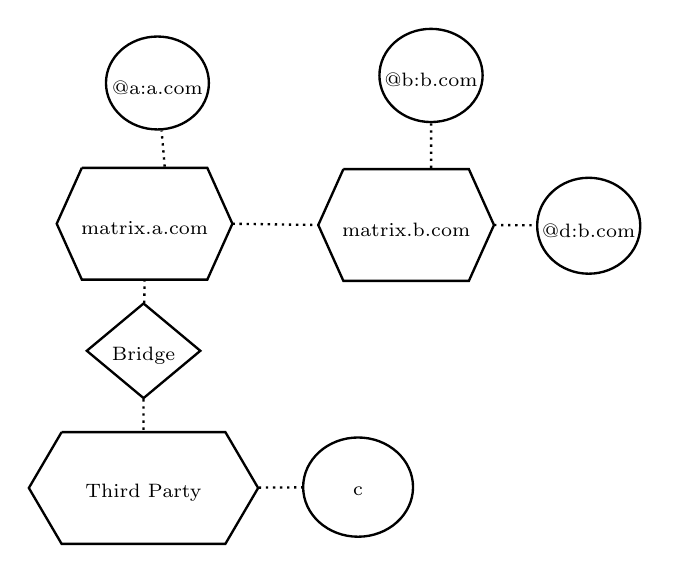
\begin{tikzpicture}
\pgftransformxscale{1.000000}
\pgftransformyscale{-1.000000}
\definecolor{dialinecolor}{rgb}{0.000000, 0.000000, 0.000000}
\pgfsetstrokecolor{dialinecolor}
\definecolor{dialinecolor}{rgb}{1.000000, 1.000000, 1.000000}
\pgfsetfillcolor{dialinecolor}
\pgfsetlinewidth{0.100000\du}
\pgfsetdash{}{0pt}
\pgfsetdash{}{0pt}
\pgfsetbuttcap
\pgfsetmiterjoin
\pgfsetlinewidth{0.100000\du}
\pgfsetbuttcap
\pgfsetmiterjoin
\pgfsetdash{}{0pt}
\definecolor{dialinecolor}{rgb}{1.000000, 1.000000, 1.000000}
\pgfsetfillcolor{dialinecolor}
\pgfpathmoveto{\pgfpoint{12.307500\du}{9.250000\du}}
\pgfpathlineto{\pgfpoint{17.642500\du}{9.250000\du}}
\pgfpathlineto{\pgfpoint{18.709500\du}{11.625000\du}}
\pgfpathlineto{\pgfpoint{17.642500\du}{14.000000\du}}
\pgfpathlineto{\pgfpoint{12.307500\du}{14.000000\du}}
\pgfpathlineto{\pgfpoint{11.240500\du}{11.625000\du}}
\pgfpathlineto{\pgfpoint{12.307500\du}{9.250000\du}}
\pgfusepath{fill}
\definecolor{dialinecolor}{rgb}{0.000000, 0.000000, 0.000000}
\pgfsetstrokecolor{dialinecolor}
\pgfpathmoveto{\pgfpoint{12.307500\du}{9.250000\du}}
\pgfpathlineto{\pgfpoint{17.642500\du}{9.250000\du}}
\pgfpathlineto{\pgfpoint{18.709500\du}{11.625000\du}}
\pgfpathlineto{\pgfpoint{17.642500\du}{14.000000\du}}
\pgfpathlineto{\pgfpoint{12.307500\du}{14.000000\du}}
\pgfpathlineto{\pgfpoint{11.240500\du}{11.625000\du}}
\pgfpathlineto{\pgfpoint{12.307500\du}{9.250000\du}}
\pgfusepath{stroke}
% setfont left to latex
\definecolor{dialinecolor}{rgb}{0.000000, 0.000000, 0.000000}
\pgfsetstrokecolor{dialinecolor}
\node at (14.975000\du,11.819062\du){\scriptsize{matrix.a.com}};
\pgfsetlinewidth{0.100000\du}
\pgfsetdash{}{0pt}
\pgfsetdash{}{0pt}
\pgfsetbuttcap
\pgfsetmiterjoin
\pgfsetlinewidth{0.100000\du}
\pgfsetbuttcap
\pgfsetmiterjoin
\pgfsetdash{}{0pt}
\definecolor{dialinecolor}{rgb}{1.000000, 1.000000, 1.000000}
\pgfsetfillcolor{dialinecolor}
\pgfpathmoveto{\pgfpoint{23.426800\du}{9.305000\du}}
\pgfpathlineto{\pgfpoint{28.761800\du}{9.305000\du}}
\pgfpathlineto{\pgfpoint{29.828800\du}{11.680000\du}}
\pgfpathlineto{\pgfpoint{28.761800\du}{14.055000\du}}
\pgfpathlineto{\pgfpoint{23.426800\du}{14.055000\du}}
\pgfpathlineto{\pgfpoint{22.359800\du}{11.680000\du}}
\pgfpathlineto{\pgfpoint{23.426800\du}{9.305000\du}}
\pgfusepath{fill}
\definecolor{dialinecolor}{rgb}{0.000000, 0.000000, 0.000000}
\pgfsetstrokecolor{dialinecolor}
\pgfpathmoveto{\pgfpoint{23.426800\du}{9.305000\du}}
\pgfpathlineto{\pgfpoint{28.761800\du}{9.305000\du}}
\pgfpathlineto{\pgfpoint{29.828800\du}{11.680000\du}}
\pgfpathlineto{\pgfpoint{28.761800\du}{14.055000\du}}
\pgfpathlineto{\pgfpoint{23.426800\du}{14.055000\du}}
\pgfpathlineto{\pgfpoint{22.359800\du}{11.680000\du}}
\pgfpathlineto{\pgfpoint{23.426800\du}{9.305000\du}}
\pgfusepath{stroke}
% setfont left to latex
\definecolor{dialinecolor}{rgb}{0.000000, 0.000000, 0.000000}
\pgfsetstrokecolor{dialinecolor}
\node at (26.094300\du,11.874062\du){\scriptsize{matrix.b.com}};
\definecolor{dialinecolor}{rgb}{1.000000, 1.000000, 1.000000}
\pgfsetfillcolor{dialinecolor}
\pgfpathellipse{\pgfpoint{15.521587\du}{5.642069\du}}{\pgfpoint{2.187187\du}{0\du}}{\pgfpoint{0\du}{1.975319\du}}
\pgfusepath{fill}
\pgfsetlinewidth{0.100000\du}
\pgfsetdash{}{0pt}
\pgfsetdash{}{0pt}
\pgfsetmiterjoin
\definecolor{dialinecolor}{rgb}{0.000000, 0.000000, 0.000000}
\pgfsetstrokecolor{dialinecolor}
\pgfpathellipse{\pgfpoint{15.521587\du}{5.642069\du}}{\pgfpoint{2.187187\du}{0\du}}{\pgfpoint{0\du}{1.975319\du}}
\pgfusepath{stroke}
% setfont left to latex
\definecolor{dialinecolor}{rgb}{0.000000, 0.000000, 0.000000}
\pgfsetstrokecolor{dialinecolor}
\node at (15.521587\du,5.836131\du){\scriptsize{@a:a.com}};
\pgfsetlinewidth{0.100000\du}
\pgfsetdash{{\pgflinewidth}{0.200000\du}}{0cm}
\pgfsetdash{{\pgflinewidth}{0.200000\du}}{0cm}
\pgfsetbuttcap
{
\definecolor{dialinecolor}{rgb}{0.000000, 0.000000, 0.000000}
\pgfsetfillcolor{dialinecolor}
% was here!!!
\definecolor{dialinecolor}{rgb}{0.000000, 0.000000, 0.000000}
\pgfsetstrokecolor{dialinecolor}
\draw (18.709500\du,11.625000\du)--(22.359800\du,11.680000\du);
}
\pgfsetlinewidth{0.100000\du}
\pgfsetdash{{\pgflinewidth}{0.200000\du}}{0cm}
\pgfsetdash{{\pgflinewidth}{0.200000\du}}{0cm}
\pgfsetbuttcap
{
\definecolor{dialinecolor}{rgb}{0.000000, 0.000000, 0.000000}
\pgfsetfillcolor{dialinecolor}
% was here!!!
\definecolor{dialinecolor}{rgb}{0.000000, 0.000000, 0.000000}
\pgfsetstrokecolor{dialinecolor}
\draw (15.831059\du,9.199912\du)--(15.697207\du,7.661089\du);
}
\pgfsetlinewidth{0.100000\du}
\pgfsetdash{}{0pt}
\pgfsetdash{}{0pt}
\pgfsetbuttcap
\pgfsetmiterjoin
\pgfsetlinewidth{0.100000\du}
\pgfsetbuttcap
\pgfsetmiterjoin
\pgfsetdash{}{0pt}
\definecolor{dialinecolor}{rgb}{1.000000, 1.000000, 1.000000}
\pgfsetfillcolor{dialinecolor}
\pgfpathmoveto{\pgfpoint{11.448100\du}{20.483700\du}}
\pgfpathlineto{\pgfpoint{18.410600\du}{20.483700\du}}
\pgfpathlineto{\pgfpoint{19.803100\du}{22.858700\du}}
\pgfpathlineto{\pgfpoint{18.410600\du}{25.233700\du}}
\pgfpathlineto{\pgfpoint{11.448100\du}{25.233700\du}}
\pgfpathlineto{\pgfpoint{10.055600\du}{22.858700\du}}
\pgfpathlineto{\pgfpoint{11.448100\du}{20.483700\du}}
\pgfusepath{fill}
\definecolor{dialinecolor}{rgb}{0.000000, 0.000000, 0.000000}
\pgfsetstrokecolor{dialinecolor}
\pgfpathmoveto{\pgfpoint{11.448100\du}{20.483700\du}}
\pgfpathlineto{\pgfpoint{18.410600\du}{20.483700\du}}
\pgfpathlineto{\pgfpoint{19.803100\du}{22.858700\du}}
\pgfpathlineto{\pgfpoint{18.410600\du}{25.233700\du}}
\pgfpathlineto{\pgfpoint{11.448100\du}{25.233700\du}}
\pgfpathlineto{\pgfpoint{10.055600\du}{22.858700\du}}
\pgfpathlineto{\pgfpoint{11.448100\du}{20.483700\du}}
\pgfusepath{stroke}
% setfont left to latex
\definecolor{dialinecolor}{rgb}{0.000000, 0.000000, 0.000000}
\pgfsetstrokecolor{dialinecolor}
\node at (14.929350\du,23.052763\du){\scriptsize{Third Party}};
\definecolor{dialinecolor}{rgb}{1.000000, 1.000000, 1.000000}
\pgfsetfillcolor{dialinecolor}
\fill (14.932210\du,15.015800\du)--(17.344719\du,17.026867\du)--(14.932210\du,19.037933\du)--(12.519700\du,17.026867\du)--cycle;
\pgfsetlinewidth{0.100000\du}
\pgfsetdash{}{0pt}
\pgfsetdash{}{0pt}
\pgfsetmiterjoin
\definecolor{dialinecolor}{rgb}{0.000000, 0.000000, 0.000000}
\pgfsetstrokecolor{dialinecolor}
\draw (14.932210\du,15.015800\du)--(17.344719\du,17.026867\du)--(14.932210\du,19.037933\du)--(12.519700\du,17.026867\du)--cycle;
% setfont left to latex
\definecolor{dialinecolor}{rgb}{0.000000, 0.000000, 0.000000}
\pgfsetstrokecolor{dialinecolor}
\node at (14.932210\du,17.220929\du){\scriptsize{Bridge}};
\pgfsetlinewidth{0.100000\du}
\pgfsetdash{{\pgflinewidth}{0.200000\du}}{0cm}
\pgfsetdash{{\pgflinewidth}{0.200000\du}}{0cm}
\pgfsetbuttcap
{
\definecolor{dialinecolor}{rgb}{0.000000, 0.000000, 0.000000}
\pgfsetfillcolor{dialinecolor}
% was here!!!
\definecolor{dialinecolor}{rgb}{0.000000, 0.000000, 0.000000}
\pgfsetstrokecolor{dialinecolor}
\draw (14.961006\du,14.989865\du)--(14.975000\du,14.000000\du);
}
\pgfsetlinewidth{0.100000\du}
\pgfsetdash{{\pgflinewidth}{0.200000\du}}{0cm}
\pgfsetdash{{\pgflinewidth}{0.200000\du}}{0cm}
\pgfsetbuttcap
{
\definecolor{dialinecolor}{rgb}{0.000000, 0.000000, 0.000000}
\pgfsetfillcolor{dialinecolor}
% was here!!!
\definecolor{dialinecolor}{rgb}{0.000000, 0.000000, 0.000000}
\pgfsetstrokecolor{dialinecolor}
\draw (14.930476\du,19.086535\du)--(14.929300\du,20.483700\du);
}
\definecolor{dialinecolor}{rgb}{1.000000, 1.000000, 1.000000}
\pgfsetfillcolor{dialinecolor}
\pgfpathellipse{\pgfpoint{24.052157\du}{22.821607\du}}{\pgfpoint{2.335657\du}{0\du}}{\pgfpoint{0\du}{2.109407\du}}
\pgfusepath{fill}
\pgfsetlinewidth{0.100000\du}
\pgfsetdash{}{0pt}
\pgfsetdash{}{0pt}
\pgfsetmiterjoin
\definecolor{dialinecolor}{rgb}{0.000000, 0.000000, 0.000000}
\pgfsetstrokecolor{dialinecolor}
\pgfpathellipse{\pgfpoint{24.052157\du}{22.821607\du}}{\pgfpoint{2.335657\du}{0\du}}{\pgfpoint{0\du}{2.109407\du}}
\pgfusepath{stroke}
% setfont left to latex
\definecolor{dialinecolor}{rgb}{0.000000, 0.000000, 0.000000}
\pgfsetstrokecolor{dialinecolor}
\node at (24.052157\du,23.015670\du){\scriptsize{c}};
\pgfsetlinewidth{0.100000\du}
\pgfsetdash{{\pgflinewidth}{0.200000\du}}{0cm}
\pgfsetdash{{\pgflinewidth}{0.200000\du}}{0cm}
\pgfsetbuttcap
{
\definecolor{dialinecolor}{rgb}{0.000000, 0.000000, 0.000000}
\pgfsetfillcolor{dialinecolor}
% was here!!!
\definecolor{dialinecolor}{rgb}{0.000000, 0.000000, 0.000000}
\pgfsetstrokecolor{dialinecolor}
\draw (19.831825\du,22.841858\du)--(21.666161\du,22.833056\du);
}
\definecolor{dialinecolor}{rgb}{1.000000, 1.000000, 1.000000}
\pgfsetfillcolor{dialinecolor}
\pgfpathellipse{\pgfpoint{27.152151\du}{5.321566\du}}{\pgfpoint{2.193451\du}{0\du}}{\pgfpoint{0\du}{1.980976\du}}
\pgfusepath{fill}
\pgfsetlinewidth{0.100000\du}
\pgfsetdash{}{0pt}
\pgfsetdash{}{0pt}
\pgfsetmiterjoin
\definecolor{dialinecolor}{rgb}{0.000000, 0.000000, 0.000000}
\pgfsetstrokecolor{dialinecolor}
\pgfpathellipse{\pgfpoint{27.152151\du}{5.321566\du}}{\pgfpoint{2.193451\du}{0\du}}{\pgfpoint{0\du}{1.980976\du}}
\pgfusepath{stroke}
% setfont left to latex
\definecolor{dialinecolor}{rgb}{0.000000, 0.000000, 0.000000}
\pgfsetstrokecolor{dialinecolor}
\node at (27.152151\du,5.515629\du){\scriptsize{@b:b.com}};
\definecolor{dialinecolor}{rgb}{1.000000, 1.000000, 1.000000}
\pgfsetfillcolor{dialinecolor}
\pgfpathellipse{\pgfpoint{33.856191\du}{11.710625\du}}{\pgfpoint{2.191191\du}{0\du}}{\pgfpoint{0\du}{2.039375\du}}
\pgfusepath{fill}
\pgfsetlinewidth{0.100000\du}
\pgfsetdash{}{0pt}
\pgfsetdash{}{0pt}
\pgfsetmiterjoin
\definecolor{dialinecolor}{rgb}{0.000000, 0.000000, 0.000000}
\pgfsetstrokecolor{dialinecolor}
\pgfpathellipse{\pgfpoint{33.856191\du}{11.710625\du}}{\pgfpoint{2.191191\du}{0\du}}{\pgfpoint{0\du}{2.039375\du}}
\pgfusepath{stroke}
% setfont left to latex
\definecolor{dialinecolor}{rgb}{0.000000, 0.000000, 0.000000}
\pgfsetstrokecolor{dialinecolor}
\node at (33.856191\du,11.904688\du){\scriptsize{@d:b.com}};
\pgfsetlinewidth{0.100000\du}
\pgfsetdash{{\pgflinewidth}{0.200000\du}}{0cm}
\pgfsetdash{{\pgflinewidth}{0.200000\du}}{0cm}
\pgfsetbuttcap
{
\definecolor{dialinecolor}{rgb}{0.000000, 0.000000, 0.000000}
\pgfsetfillcolor{dialinecolor}
% was here!!!
\definecolor{dialinecolor}{rgb}{0.000000, 0.000000, 0.000000}
\pgfsetstrokecolor{dialinecolor}
\draw (29.828800\du,11.680000\du)--(31.618315\du,11.693608\du);
}
\pgfsetlinewidth{0.100000\du}
\pgfsetdash{{\pgflinewidth}{0.200000\du}}{0cm}
\pgfsetdash{{\pgflinewidth}{0.200000\du}}{0cm}
\pgfsetbuttcap
{
\definecolor{dialinecolor}{rgb}{0.000000, 0.000000, 0.000000}
\pgfsetfillcolor{dialinecolor}
% was here!!!
\definecolor{dialinecolor}{rgb}{0.000000, 0.000000, 0.000000}
\pgfsetstrokecolor{dialinecolor}
\draw (27.157811\du,9.254838\du)--(27.155073\du,7.352431\du);
}
\end{tikzpicture}
